Para probar la funcionalidad de nuestro parser primogénito creamos los siguientes tests que abarcan las funcionalidades provistas por el lenguaje.

\subsection{Test de funcionalidades básicas}
	El código se encuentra en testsPropios/testBueno1.cod
	\lstinputlisting{testsPropios/testBueno1.cod}
	Salida:
	\lstinputlisting{testsPropios/salidaTest1.out}

Como sus comentarios lo indican, este test permite probar algunas de las funcionalidades básicas computando la función de Fibonacci.

\subsection{Test de más funcionalidades}
	El código se encuentra en testsPropios/testBueno2.cod
	\lstinputlisting{testsPropios/testBueno2.cod}
	Salida:
	\lstinputlisting{testsPropios/salidaTest2.out}
	
Ambos tests dan el siguiente gráfico, como era esperado:

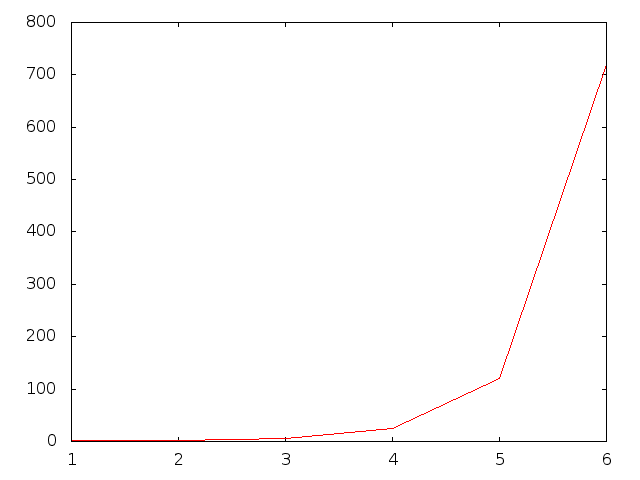
\includegraphics[width=0.60\textwidth,height=0.60\textheight,keepaspectratio]{testsPropios/graficoTest1.png}
\subsection{Tests de desambiguación}
	El código se encuentra en testsPropios/testBueno3.cod
	\lstinputlisting{testsPropios/testBueno3.cod}
	Salida:
	\lstinputlisting{testsPropios/salidaTest3.out}
	
	En este ejemplo vemos cómo resolvimos el problema de la desambiguación de los ifthenelse anidados. Nuestro enfoque es el mismo que el útilizado en lenguajes de programación conocidos como C o C++. Podemos ver un ejemplo con el siguiente código:
		\lstinputlisting{testsPropios/pruebaIfThenElse.c}
	
	Para garantizar dicho funcionamiento no hizo falta modificar nada. Ante el conflicto Shift-Reduce BISON elige siempre Shift por defecto, con lo cual el resultado es el esperado.
	
	\textbf{Nota}: El conflicto redunda en un Shift-Reduce porque nuestra gramática presenta una ambigüedad: al encontrar el segundo $else$ como lookahead BISON no sabe si aplicar un Reduce (reducir el código del $if$ más interno a un símbolo $IfThen$ y ``asociar'' luego el $else$ al $if$ externo) o un Shift (consumir el $else$ con su bloque de código para después reducir el $if$ lo más interno a un símbolo $IfThenElse$ y el más externo a un $IfThen$).